% From the Research Methods workbook, page 242.
%
%% This section explains how the research was performed.
% Sometimes it has a different name (e.g., ‘Experiments’), but still has
% the same purpose: to describe the methods. The section should
% allow another researcher to replicate the study (i.e., perform it
% again). This is different from obtaining the same findings). In
% psychology, this section has subsections describing participants,
% design, stimuli, procedure, and data analysis.

This project will follow a design research methodology \citep{wieringa2014design}, consisting of iterative cycles of building, testing, and refining artifacts.
The artifact in this case is a guardrail mechanism for LLMs that constrains or validates generated output.

We will test and compare four experimental conditions to evaluate the effectiveness of different guardrail approaches for ensuring correctness in medical prompts:

\begin{itemize}
    \item \textbf{Baseline:} No guardrails applied.
    \item \textbf{RAG-only:} Responses are grounded in external verified medical sources using retrieval-augmented generation \citep{dong2024guardrails}.
    \item \textbf{Moderator-only:} A second AI model evaluates the generated output and flags or blocks incorrect or unsafe content \citep{inan2023llamaguard}.
    \item \textbf{Combined:} Both RAG and moderator-AI are applied sequentially, checking it with both methods.
\end{itemize}

The evaluation focuses on whether the guardrail meets defined correctness criteria in realistic scenarios and what design choices contribute to its effectiveness.

\subsection{Baseline setup}
In the baseline setup (figure \ref{fig:baselineSetup}) we will use a large language model (LLM) to generate responses to medical prompts without any guardrails.
The model used is the Google Gemini 2.0 flash model, which is a large language model trained on a wide range of data, including medical texts \citep{saab2024capabilities}.
The medical question will be directly used as prompt for the LLM.
Later iterations of the project proved that the medical question needed to be extended with additional patient information.
The information was primarily needed for manual review by an expert user as the medical context of the patient is important to validate if the recipe is correct.
Together with the prompt the LLM wil be provided with a system instruction that specifies the task and expected output format.
As the medical question if formulated in Dutch, the system instruction is also in Dutch.
\begin{verbatim}
    Je bent een medisch expert. Beantwoord de medische vraag met
    een recept volgens het volgende template:
    'Rp. [Medicijnaam] [Sterkte] [Vorm]\ndtd. No. [Aantal]\n S. [Instructie]'.
    Neem relevante informatie over de patiënt in acht, zoals leeftijd en
    eventuele allergieën.
    Geef de formele medicijnnaam in het JSON-veld 'medicijn'.
    Benoem de categorie van het medicijn in het JSON-veld 'categorie'.
    Geef bij de instructie ook de duur van de behandeling aan.
    Herhaal de medische vraag in het JSON-veld 'medische_vraag'.
    Voeg de patiëntinformatie toe in het JSON-veld 'patientinformatie'.
\end{verbatim}

\begin{figure}[H]
    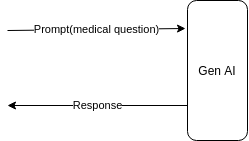
\includegraphics[width=0.5\textwidth]{figures/baselineSetup.png}
    \captionof{figure}{Baseline setup for generating medical recipes without guardrails.}
    \label{fig:baselineSetup}
\end{figure}

\subsection{RAG-only setup}

In the RAG-only setup \ref{fig:ragSetup}, we will use a large language model (LLM) to generate responses to medical prompts, but with the addition of retrieval-augmented generation (RAG).
The RAG component will retrieve relevant information about the medication from apotheek.nl and use that information to validate the generated output.
The output will be validated for correctness of indication, dosage, frequency and duration of use.
When the output is not correct the response will be blocked. Only when the output is correct, it will be returned to the user.

\begin{figure}[H]
    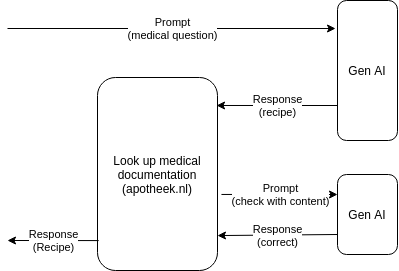
\includegraphics[width=0.5\textwidth]{figures/RAGSetup.png}
    \captionof{figure}{RAG-only setup for generating medical recipes with retrieval-augmented generation.}
    \label{fig:ragSetup}
\end{figure}

\subsection{Moderator-only setup}

In the moderator-only setup \ref{fig:moderatorSetup}, we will use a large language model (LLM) to generate responses to medical prompts, but with the addition of a moderator model.
The moderator model will evaluate the generated output and flag or block incorrect or unsafe content.
The same model will be used for both the generation and moderation tasks, but with different system instructions.

\begin{figure}[H]
    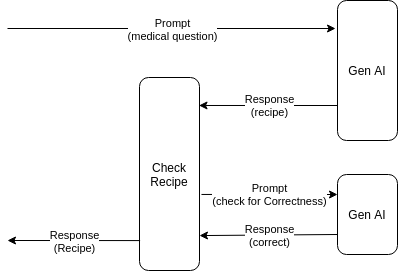
\includegraphics[width=0.5\textwidth]{figures/moderatorSetup.png}
    \captionof{figure}{Moderator-only setup for generating medical recipes with a moderator model.}
    \label{fig:moderatorSetup}
\end{figure}

\subsection{Combined setup}

In the combined setup \ref{fig:combinedSetup}, we will use a large language model (LLM) to generate responses to medical prompts, with both retrieval-augmented generation (RAG) and a moderator model.
The RAG component will retrieve relevant information about the medication from apotheek.nl and use that information to validate the generated output.
The moderator model will then evaluate the generated output and flag or block incorrect or unsafe content.
The recipe is considered correct when it is both grounded in the retrieved information and passes the moderation check.

\begin{figure}[H]
    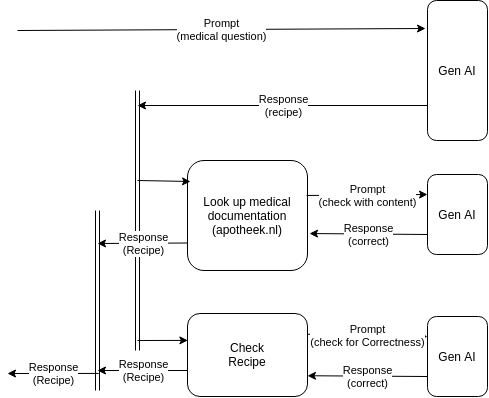
\includegraphics[width=0.5\textwidth]{figures/combinedSetup.png}
    \captionof{figure}{Combined setup for generating medical recipes with retrieval-augmented generation and a moderator model.}
    \label{fig:combinedSetup}
\end{figure}

\subsection{Apparatus}

The exact technical setup for this project has not yet been determined. An initial idea is to use existing large language model agents, such as ChatGPT with function-calling capabilities, to simulate retrieval-augmented generation and moderation behaviors without requiring full custom implementation in Python.

If this approach proves insufficient for the intended experiments, alternative methods will be explored. Possible options include low-code or API-based solutions, or minimal programming to construct basic prototypes.

The final choice of tools and models will depend on feasibility, ease of integration, and their suitability for testing correctness guardrails in medical prompts.

\subsection{Stimuli}

To evaluate the guardrails, we will use a fixed set of prompts that represent high-risk medical questions, particularly about medications (e.g., dosage, indications, and contraindications).
These tasks represent real-world LLM use cases with identifiable correctness constraints \citep{pais2024medication}.
The responses will be formatted as formal medical recipes following the Dutch guidelines for medication prescriptions \citep{farmacotherapeutischkompas}.
\begin{verbatim}
        Rp.   [Medicijnnaam] [Sterkte] [Vorm]
          dtd. No. [Aantal]
          S. [Instructie]
\end{verbatim}

\subsection{Dataset}

The dataset will consist of a set of medical questions and their corresponding correct and incorrect recipes.
The medical questions will be used as prompt input for the LLMs, and the recipes will be used to evaluate the correctness of the generated output.
Because recipes are subject to privacy regulations, the dataset is completely synthetic and has been generated by the researchers.
If this research was executed beyond the scope of a course, we would have used real-world data from the Dutch guidelines for medication prescriptions \citep{farmacotherapeutischkompas}.
The medical questions would have been anonymized, and the recipes would have been generated by a medical professional.
For this course context we will restrict ourselves to the fictional dataset.
To make sure the dataset is representative of real-world medical questions a 1\% sample of the dataset will be manually checked by a medical professional.

The dataset has 2000 examples of medical questions and their corresponding recipes.
For test purposes a secondary dataset is created with the based on the examples, but with deliberately incorrect recipes or medical questions.
The test set is restricted to 500 examples.
The guardrail performance can be measured by comparing the number of recipes that get blocked by the guardrail mechanism.
Blocking a valid recipe results in a false positive, while allowing an incorrect recipe to pass through results in a false negative.
Appendix \ref{appendix:dataset} provides an example of the two datasets.

\subsection{Design}

Each condition will be tested across the same prompt set.
Performance will be evaluated in terms of correctness, safety, and response quality.
Correctness of the output will be validated against the available medication guidelines available in the ``Farmacotherapeutisch Kompas'' \citep{farmacotherapeutischkompas} and the ``Geneesmiddeleninformatiebank'' \citep{geneesmiddeleninformatiebank}.
The design is iterative, allowing refinements to each method across evaluation cycles.
Each cycle will test the correctness of a medical prompt based on datasets correct and incorrect medical recipes.
The same dataset will be used for all four conditions, ensuring a fair comparison.

\subsection{Procedure}

\begin{enumerate}
    \item Identify output correctness criteria for selected medical prompts.
    \item Implement guardrail mechanisms: RAG, moderator model, and their combination.
    \item For each prompt, generate model outputs in four conditions: Baseline, RAG-only, Moderator-only, and Combined.
    \item Compare outputs against correctness criteria using expert annotation or rule-based validation.
    \item Analyze failures, compare effectiveness, and refine guardrail designs.
\end{enumerate}

\subsection{Data analysis}

Each guardrail condition (Baseline, RAG-only, Moderator-only, Combined) will be evaluated using the following metrics:

\begin{itemize}
    \item \textbf{Error rate:} Percentage of incorrect or unsafe answers.
    \item \textbf{Precision/Recall:} For detecting unsafe or medically incorrect outputs.
    \item \textbf{False positives / negatives:} Analysis of over- or under-blocking.
    \item \textbf{Qualitative analysis:} Categorization of failure types per condition.
    \item \textbf{Reflective analysis:} Documentation of design choices and their impact.
\end{itemize}

This comparison allows us to determine whether a specific approach—or their combination—can achieve 100\% correctness or significantly reduce critical errors.
